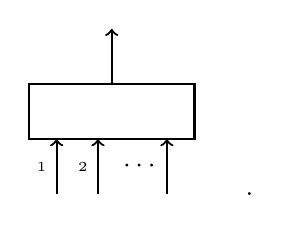
\begin{tikzpicture}[scale=0.35, thick] % , baseline = -3.5pt

\draw[->] (2,-1)--(2,1) node[midway,right] {\tiny ${\exformula}$};
\draw (-1,-1) rectangle (5,-3);
\node[anchor=center] (text) at (2,-2) {\small $\bencodingof{\exformula}$};
\draw[<-] (0,-3)--(0,-5) node[midway,left] {\tiny $\catvariableof{1}$};
\draw[<-] (1.5,-3)--(1.5,-5) node[midway,left] {\tiny $\catvariableof{2}$};
\node[anchor=center] (text) at (3,-4) {$\cdots$};
\draw[<-] (4,-3)--(4,-5) node[midway,right] {\tiny $\catvariableof{\atomorder}$};

\node[anchor=center] (text) at (7,-5) {$.$};

\end{tikzpicture}